\lecture{14}{9 April.}{}
\begin{eg}
    If \(X\) is a continuous random variable with 
    \[
        f_X(t) = \begin{dcases}
            \frac{C}{t^3}, &\text{ if } t \ge 1 ;\\
            0, &\text{ if } t < 1.
        \end{dcases}
    \]
    \begin{itemize}
        \item [(1)] What is \(C\)?
        \item [(2)] What are \(\mathbb{E} [X]\) and \(\Var(X)\)?  
    \end{itemize}
\end{eg}

\begin{explanation}
    \hfill 
    \begin{itemize}
        \item [(1)] We have \(\int _{-\infty }^{\infty } f_X(t) \, \mathrm{d} t = 1 \), so 
        \[
            1 = \int _{-\infty }^1 f_X(t) \, \mathrm{d} t + \int _{1}^{\infty} f_X(t) \, \mathrm{d} t = \int _{1}^{\infty} f_X(t) \, \mathrm{d} t = \frac{C}{2},  
        \]
        so \(C = 2\).
        \item [(2)]
        \[
            \mathbb{E} [X] = \int _{-\infty }^{\infty } t f_X(t) \, \mathrm{d} t = \int _1^{\infty } t f_X(t) \, \mathrm{d} t = 2.  
        \]
        \begin{align*}
            \Var(X) &= \mathbb{E} [X^2] - \mathbb{E} [X]^2 = \int _{-\infty }^{\infty } t^2 f_X(t) \, \mathrm{d} t - 4 = \int _1^{\infty } t^2 \cdot \frac{2}{t^3} \, \mathrm{d} t - 4 = \infty,  
        \end{align*}
        so \(\Var(X)\) does not exist. 
    \end{itemize}
\end{explanation}

\begin{remark}
    The divergence of the variance or even the expectation can also occur for discrete random variables when the probability of large values doesn't decay very quickly, e.g. \(\mathbb{P} (X = k) = \frac{c}{k^2}\) for \(k \in \mathbb{N} \).  
\end{remark}

\section{Continuous Probability Distribution}
\subsection{Uniform Distribution}
\begin{definition}[Uniform Distribution]
    Suppose \(\alpha < \beta \in \mathbb{R}\), then we say \(X \sim \mathrm{Unif}(\alpha , \beta ) \) if we want to choose a uniformly random point in \([\alpha , \beta ]\), and \(X\) is the outcome. Note that the probability of a subinterval of \([\alpha , \beta ]\) only depends on its width.      
\end{definition}

\paragraph{PDF}
\[
    f_X(t) = \begin{dcases}
        C, &\text{ if } t \in [\alpha , \beta] ;\\
        0, &\text{ if } t \notin [\alpha , \beta] 
    \end{dcases}
\]
since the probability of every point in \([\alpha , \beta]\) to be choose is same. Now we compute \(C\). Note that 
\[
    1 = \int _{-\infty }^{\infty } f_X(t) \, \mathrm{d} t = \int _\alpha ^\beta C \, \mathrm{d} t = C(\beta - \alpha ),  
\] 
so \(C = \frac{1}{\beta - \alpha}\).

\paragraph{CDF}
\begin{align*}
    F_X(x) &= \mathbb{P} (X \le x) = \int _{-\infty }^{x} f_X(t) \, \mathrm{d} t = \begin{dcases}
        0, &\text{ if } x \le \alpha ;\\
        \int _{\alpha }^x \frac{1}{\beta - \alpha } \, \mathrm{d} t = \frac{x - \alpha}{\beta - \alpha} , &\text{ if } \alpha \le x \le \beta;\\
        1, &\text{ if } x \ge \beta .
    \end{dcases} 
\end{align*}

\paragraph{Expectation}
\[
    \mathbb{E} [X] = \int _{-\infty }^{\infty } t f_X(t) \, \mathrm{d} t = \int _\alpha ^\beta \frac{t}{\beta - \alpha} \, \mathrm{d} t = \frac{\alpha + \beta}{2}.  
\]

\paragraph{Variance}
We know \(\Var(X) = \mathbb{E} [X^2] - \mathbb{E} [X]^2\), where 
\begin{align*}
    \mathbb{E} [X^2] &= \int _{-\infty }^{\infty} t^2 f_X(t) \, \mathrm{d} t = \int _{\alpha }^{\beta } \frac{t^2}{\beta - \alpha } \, \mathrm{d} t = \frac{\beta ^2 + \alpha \beta + \alpha ^2}{3}.  \\
    \mathbb{E} [X]^2 &= \left( \frac{\alpha + \beta}{2} \right)^2 = \frac{\beta ^2 + 2 \alpha \beta + \alpha ^2}{4}. 
\end{align*} 

Hence,
\[
    \Var(X) =\frac{\beta ^2 + \alpha \beta + \alpha ^2}{3} - \frac{\beta ^2 + 2 \alpha \beta + \alpha ^2}{4} = \frac{(\beta - \alpha)^2}{12}.
\]

\begin{theorem}[Simulating continuous random variables]
    Let \(X\) be a continuous random variable with cdf \(F_X: \mathbb{R} \to [0, 1]\). Let \(U \sim \mathrm{Unif}(0, 1) \). Let \(Y = F_X^{-1}(U) \in \mathbb{R}\). Then \(Y\) has the same distribution as \(X\).      
\end{theorem}

\begin{proof}
    We want to show \(F_Y = F_X\). Then,
    \begin{align*}
        F_Y(x) &= \mathbb{P} (Y \le x) = \mathbb{P} (F_X^{-1}(U) \le x) = \mathbb{P} (U \le F_X(x)) = F_U(F_X(x)) = \frac{F_X(x) - 0}{1 - 0} = F_X(x)
    \end{align*} 
    because \(F_X\) is increasing and \(U \sim \mathrm{Unif}(0, 1) \). 
\end{proof}

\subsection{Exponential Distribution}
Setting: A bus arrives at a bus stop on average every \(18\) minutes. We arrive at the bus stops. How long do we have to wait for the next bus?

If \(X\) is our waiting time, we want \(X\) to satisfy memoryless property:
\[
    \mathbb{P} (X \ge x+y \mid X \ge x) = \mathbb{P} (X \ge y).
\]  

\begin{theorem}
    The only continuous memoryless distribution is the exponential distribution.
\end{theorem}

\begin{proof}
    Let \(X\) be a memoryless continuous distribution. Define \(g(x) = \mathbb{P} (X \ge x)\). Then,
    \[
        g(x + y) = \mathbb{P} (X \ge x+y) = \mathbb{P} (X \ge x+y \mid X \ge x) \mathbb{P} (X \ge x) = \mathbb{P} (X \ge y) \mathbb{P} (X \ge x) = g(y) g(x).
    \]  
    Thus, \(g(x + y) = g(x) g(y)\) for all \(x, y \ge 0\). Now define \(\lambda = - \ln (g(1))\), i.e. \(g(1) = e^{-\lambda}\). Since \(g(1) = \mathbb{P} (X \ge 1) \in [0, 1]\), so \(\lambda \in [0, \infty)\). Let \(n \in \mathbb{N}\), then 
    \[
        g(n) = g(1 + 1 + \dots + 1) = g(1)^n = e^{-n \lambda}.
    \]      
    Let \(\frac{r}{s} \in \mathbb{Q} _{\ge 0}\), then 
    \[
        g(r) = g\left( \frac{r}{s} + \frac{r}{s} + \dots + \frac{r}{s} \right) = g \left( \frac{r}{s} \right)^s,  
    \]
    so \(g\left( \frac{r}{s} \right) = g(r)^{\frac{1}{s}} = (e^{-r \lambda})^{\frac{1}{s}}= e^{-\lambda \frac{r}{s}}\). Now let \(x \in \mathbb{R}\), let \(q_n\) be a sequence of rational numbers with \(q_n \searrow x\). Then,
    \begin{align*}
        g(x) &= \mathbb{P} (X \ge x) = 1 - \mathbb{P} (X \le x) = 1 - \lim_{n \to \infty} \mathbb{P} (X \le q_n) = \lim_{n \to \infty} \mathbb{P} (X > q_n) = \lim_{n \to \infty} g(q_n) \\ &= \lim_{n \to \infty} e^{-\lambda q_n} = e^{-\lambda x}.
    \end{align*}
\end{proof}

\begin{notation}
    We say \(X \sim \mathrm{Exp}(\lambda) \) for \(\lambda \in \mathbb{R} _{> 0}\) if \(X\) is of exponential distribution. 
\end{notation}

\paragraph{CDF}
\[
    F_X(x) = \mathbb{P} (X \le x) = \begin{dcases}
            1 - e^{-\lambda x}, &\text{ if } x \ge 0 ;\\
            0, &\text{ if } x < 0.
        \end{dcases}
\]

\paragraph{PDF}
\[
    f_X(t) = F_X^{\prime} (t) = \begin{dcases}
        \lambda e^{-\lambda t}, &\text{ if } t > 0 ;\\
        0, &\text{ if } t \le 0.
    \end{dcases}
\]

\paragraph{Expectation}
\begin{align*}
    \mathbb{E} [X] &= \int _{-\infty }^{\infty } t f_X(t) \, \mathrm{d} t = \int _0^{\infty} t \lambda e^{-\lambda t} \, \mathrm{d} t \\
    &= [t(-e^{-\lambda t})]_0^{\infty} - \int _0^{\infty} (-e^{-\lambda t})\, \mathrm{d} t = \int _0^{\infty } e^{-\lambda t} \, \mathrm{d} t = \left[ \frac{-e^{-\lambda t}}{\lambda } \right]_0^{\infty}.     
\end{align*}

Hence, \(\mathbb{E} [X] = \frac{1}{\lambda}\). 

\paragraph{Variation}
Since \(\Var(X) = \mathbb{E} [X^2] - \mathbb{E} [X]^2\), where 
\begin{align*}
    \mathbb{E} [X^2] &= \int _{-\infty }^{\infty} t^2 f_X(t) \, \mathrm{d} t = \int _0^{\infty } t^2 \lambda e^{-\lambda t} \, \mathrm{d} t = \frac{2}{\lambda ^2}.  
\end{align*} 
Thus,
\[
    \mathbb{E} [X^2] - \mathbb{E} [X]^2 = \frac{2}{\lambda ^2} - \frac{1}{\lambda^2} = \frac{1}{\lambda ^2}.
\]


\begin{eg}
    A bus arrives on average every \(15\) minutes. What is the probability that we have to wait at least 5 minutes for the bus? 
\end{eg}
\begin{explanation}
    \(X \sim \mathrm{Exp}(\lambda) \), and \(\mathbb{E} [X] = \frac{1}{\lambda} = 15\), so \(\lambda = \frac{1}{15}\). Since 
    \[
        \mathbb{P} (X \ge x) = e^{-\lambda x},
    \]   
    so \(\mathbb{P} (X \ge 5) = e^{-5 \lambda } = e^{-\frac{1}{3}}\). 
\end{explanation}

\begin{eg}
    A passenger can take one of two buses. The first arrives on average every 15 minutes, the second on average every 18 minutes. If they take the first bus arrives, and the buses run independently, how long would they have to wait on average?
\end{eg}
\begin{explanation}
    Let \(X_1\) be the waiting time for the first bus, \(X_2\) be the waiting time for the second, then \(X_1 \sim \mathrm{Exp}(\frac{1}{15}) \) and \(X_2 \sim \mathrm{Exp}(\frac{1}{18}) \), then if \(W\) is the waiting time for the passenger, then \(W = \min (X_1, X_2)\). Hence,
    \begin{align*}
        F_W(x) &= \mathbb{P} (W \le x) = \mathbb{P} (\min (X_1, X_2) \le x) = 1 - \mathbb{P} (\min (X_1, X_2) > x) \\
        &= 1 - \mathbb{P} (X_1 > x \text{ and } X_2 > x) = 1 - \mathbb{P} (X_1 > x) \mathbb{P} (X_2 > x) \\
        &= 1 - (e^{-\lambda _1 x}) (e^{-\lambda _2 x}) = 1 - e^{-(\lambda _1 + \lambda _2) x},
    \end{align*}      
    where \(\lambda _1 = \frac{1}{15}\) and \(\lambda _2 = \frac{1}{18}\). Thus,
    \[
        W \sim \mathrm{Exp}(\lambda _1 + \lambda _2) = \mathrm{Exp}\left( \frac{1}{15} + \frac{1}{18} \right) = \mathrm{Exp}\left( \frac{11}{90} \right).     
    \]  
    Hence, \(\mathbb{E} [W] = \frac{90}{11}\). 

    \begin{remark}
        More generally, if \(X_i \sim \mathrm{Exp}(\lambda _i) \) for \(1 \le i \le n\), and these are independent, then 
        \[
            X = \min (X_1, X_2, \dots , X_n) \sim \mathrm{Exp} \left( \sum_{i=1}^n \lambda _i  \right).  
        \]  
    \end{remark}
\end{explanation}

\begin{eg}[Waiting Time Paradox]
   The \emph{waiting time paradox} says that if buses do \emph{not} arrive at perfectly regular intervals, then a passenger who shows up at a random time tends to land in a \emph{longer-than-average} gap between buses. Because of that sampling bias, the time the passenger waits can be larger than ``half of the average gap,'' and the bus interval that the passenger finds themself inside is also typically larger than the population-average interval.

\section*{What is going on in your example?}

Let
\[
X = \text{the time from now until the next bus arrives}.
\]
If we model the bus arrivals as a Poisson process with rate $\lambda = 1/10$ per minute, then
\[
X \sim \mathrm{Exp}(1/10),
\qquad
\mathbb{E}[X] = 10 \text{ minutes.}
\]

Now suppose that, at the moment you observe the system,

\begin{itemize}[leftmargin=2em]
    \item the last bus left $8$ minutes ago, and
    \item the next bus will come in $2$ minutes.
\end{itemize}

So the two buses around you are exactly $10$ minutes apart.

The apparent paradox is this:

\begin{enumerate}[label=(\arabic*), leftmargin=2em]
    \item By the memoryless property, the future waiting time from \emph{now} has mean $10$ minutes.
    \item By time-reversal symmetry of the Poisson process, the elapsed time since the previous bus also has mean $10$ minutes.
    \item So it looks like
    \[
    \mathbb{E}[\text{backward gap}] + \mathbb{E}[\text{forward gap}] = 10 + 10 = 20,
    \]
    but the bus interval in the picture is only $10$ minutes.
\end{enumerate}

\section*{Where the paradox lies}

The mistake is that these expectations are \emph{not conditioned on the event that the surrounding gap equals $10$ minutes}. They are unconditional averages over \emph{all} possible observation times.

There are really two different random quantities:

\begin{itemize}[leftmargin=2em]
    \item $B$ = time since the previous bus (backward recurrence time),
    \item $F$ = time until the next bus (forward recurrence time).
\end{itemize}

For a Poisson process,
\[
B \sim \mathrm{Exp}(1/10),
\qquad
F \sim \mathrm{Exp}(1/10),
\qquad
\mathbb{E}[B] = \mathbb{E}[F] = 10.
\]

But once you are told that in this particular realization $B=8$ and $F=2$, there is nothing random left in that local picture: the surrounding interval is simply
\[
B+F=8+2=10.
\]

So the incorrect step is mixing
\[
\mathbb{E}[B] + \mathbb{E}[F]
\]
with
\[
B+F \text{ for a particular observed sample.}
\]

Those are different objects.

\section*{Why $\mathbb{E}[B+F]=20$ is actually correct}

For a Poisson bus process, the bus interval containing a \emph{random observation time} is not distributed like an ordinary interarrival time. It is \emph{length-biased}: long gaps are more likely to contain your arrival time.

If the ordinary interarrival time is
\[
T \sim \mathrm{Exp}(1/10),
\qquad
\mathbb{E}[T]=10,
\]
then the interval containing a random observation time has mean
\[
\mathbb{E}[B+F] = 20.
\]

That does \emph{not} contradict the fact that an ordinary gap between consecutive buses has average length $10$. It only says that when you sample by picking a random time, you are more likely to land inside a long gap than a short one.

For the exponential case, one can verify directly that
\[
\mathbb{E}[B+F]=\mathbb{E}[B]+\mathbb{E}[F]=10+10=20.
\]

\begin{center}
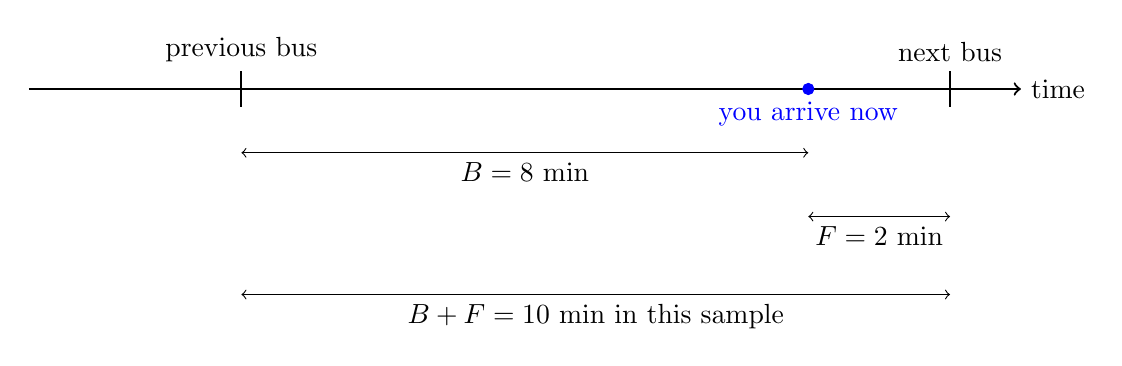
\begin{tikzpicture}[x=0.9cm,y=0.9cm]
    \draw[thick, ->] (0,0) -- (14,0) node[right] {time};
    \draw[thick] (3,-0.25) -- (3,0.25);
    \draw[thick] (13,-0.25) -- (13,0.25);
    \filldraw[blue] (11,0) circle (2pt);

    \node[above] at (3,0.25) {previous bus};
    \node[above] at (13,0.25) {next bus};
    \node[below, blue] at (11,-0.05) {you arrive now};

    \draw[<->] (3,-0.9) -- (11,-0.9);
    \node[below] at (7,-0.9) {$B=8$ min};

    \draw[<->] (11,-1.8) -- (13,-1.8);
    \node[below] at (12,-1.8) {$F=2$ min};

    \draw[<->] (3,-2.9) -- (13,-2.9);
    \node[below] at (8,-2.9) {$B+F=10$ min in this sample};
\end{tikzpicture}
\end{center}

In this drawing, the local sample gives $8+2=10$. But if you repeat the experiment many times and choose your observation time uniformly at random on a long timeline, then the average containing interval is $20$ minutes, not $10$ minutes, because long intervals are overrepresented.

\section*{Short resolution}

The paradox disappears once we separate:

\begin{itemize}[leftmargin=2em]
    \item \textbf{ordinary bus gap:} mean $10$ minutes,
    \item \textbf{gap seen by a random observer:} mean $20$ minutes,
    \item \textbf{your particular observed sample:} here it is exactly $8+2=10$ minutes.
\end{itemize}

So the statement ``$10+10=10$'' is not a real contradiction. The left side is an \emph{unconditional expectation}; the right side is the length of \emph{one realized interval} in your example. 
\end{eg}